\section{Physikalische Grundlagen}
\subsection{Strom und Spannung an Widerständen, Kondensatoren und Induktivitäten}
In diesem Versuch sind die Schaltkreise aus den Bauelementen Kondensator, Spule und Widerstand mit den Messgrößen Kapazität \(C\), Induktivität \(L\) und Widerstand \(R\) zusammengesetzt. Sie werden durch folgende Zusammenhänge zwischen Strom I und Spannung U bestimmt:

\begin{equation}
\label{1}
Widerstand\ R: U_{R}=-R\cdot I_{R}
\end{equation}
\begin{equation}
\label{2}
Kapazität\ C: I_C=-C\frac{dU_C}{dt}
\end{equation}
\begin{equation}
\label{3}
Induktivität\ L: U_{L}=-L\frac{dI_{L}}{dt}
\end{equation}

dabei sind: \vspace{0,5cm}

\begin{tabular}{l l}
\(\ U_{R}\) & := Spannung am Widerstand\\
\(\ R\)		& := Widerstand\\
\(\ I_{R}\)	& := Strom am Widerstand\\
\(\ I_{C}\)	& := Strom am Kondensator\\
\(\ C\)		& := Kapazität des Kondensators\\
\(\ \frac{dU_{C}}{dt}\)	& := Änderung der Spannung am Kondensator mit der Zeit\\
\(\ U_{L}\)	& := Spannung an der Spule\\
\(\ L\)		& := Induktivität der Spule\\
\(\ \frac{dI_{L}}{dt}\)	& := Änderung des Stroms an der Spule mit der Zeit\\
\vspace{0,5cm}
\end{tabular}\\

Die Größen R, C und L sind positiv definiert. Allerdings setzt die Beziehung zwischen Spannung und Strom aufgrund der Kirchhoff'schen Regeln ein Minuszeichen voraus denn jeder Leiter besitzt einen Widerstand, woraus eine Gegenspannung resultiert. Im Falle des Kondensators bewirkt ein positiver Strom eine Erniedrigung der Spannung und in einer Spule wird eine Spannung induziert sobald sich der Strom ändert.

\subsection{Wechselspannung an Widerständen, Kondensatoren 
Induktivitäten und Impedanzen }
\subsubsection{Wechselstrom und Wechselspannung}
Eine Wechselspannung bzw. ein Wechselstrom hat eine charakteristische sinus- oder cosinusförmige Spannung bzw. Strömung. Sie werden wie folgt bezeichnet:

\begin{equation}
\label{4}
U_{t}=U_{0}\cdot cos(\omega t+\varphi _{1})\ \ bzw.\ \ I_{t}=I_{0}\cdot cos(\omega t+\varphi _{2})
\end{equation}

Häufig werden auch komplexe Größen verwendet, da sich hierdurch viele Gleichungen vereinfachen.

\begin{equation}
\label{komplex}
U_{t}=Re \left( U_{0}\cdot e^{i\left(\omega t+\varphi _{1}\right)}\right)\ \ bzw.\ \  I_{t}=Re \left(I_{0}\cdot e^{i\left(\omega t+\varphi _{2}\right)}\right)
\end{equation}

\begin{tabular}{l l}
\(\ I_{0}\)	&	:= Maximalstrom\\
\(\ U_{0}\) &	:= Maximalspannung\\
\(\ \omega\)&	:= Kreisfrequenz\\
\(\ \varphi\)&	:= verschiedene Phasen
\end{tabular}\\

Dabei treten in Schaltkreisen mit \(R\), \(C\) und \(L\) durch Wechselspannungen Wechselströme gleicher Frequenz und Phasenverschiebungen zwischen Strom und Spannung auf. Zum Vereinfachen setzt man daher die Phase der Spannung gleich Null \(\ (\varphi _{1}=0)\) \\

\subsubsection{Impedanz Z}
Die Impedanz \(Z\) (Wechselstromwiderstand) beschreibt das Verhältnis von der Spannungs- zur Stromamplitude.

\begin{equation}
\label{5}
Z=\frac{U_{0}}{I_{0}}
\end{equation}

Setzten wir nun die Gl.\(\ \eqref{4}\) in Gl.\(\ \eqref{1}\) bis \(\ \eqref{3}\) ein, so erhalten wir die Impedanzen der Bauteile und die Phasenverschiebung des Stroms zur Spannung an R, C und L:

\begin{equation}
Z_{R}=R
\end{equation}
\begin{equation}
\varphi = \pi
\end{equation}

Für die Kondensatoren gilt des weiteren:

\begin{equation}
Z_{C}=\frac{1}{i \omega C} = \frac{-i}{\omega C}
\end{equation}
\begin{equation}
\varphi=\frac{-\pi }{2}
\end{equation}

Der Strom eilt hier der Spannung voraus. Außerdem gilt für Spulen:

\begin{equation}
Z_{L}= i \omega L\ \ und \ \ \varphi =+\frac{\pi }{2}
\end{equation}

wobei hier der Strom der Spannung hinterher läuft.

\subsubsection{Wechselstromnetzwerke}
Hier gelten die gleichen Regeln wie beim Gleichstromfall, nur dass hierfür die komplexe Impedanz benutzt wird.
Für die Reihenschaltung gilt:
\begin{equation}
Z=\mid{ \sum \limits_{i} Z_i} \mid
\end{equation}
\begin{equation}
tan \varphi ={\frac{Im \left( \sum \limits_{i} Z_{i} \right) }{Re \left( \sum \limits_{i} Z_{i} \right) }}
\end{equation}
und für die Parallelschaltung:

\begin{equation}
\frac{1}{Z}=\mid{ \sum \limits_{i} \frac{1}{Z_{i}}}\mid 
\end{equation}
\begin{equation}
tan\varphi = {\frac{Im \left( {\sum\limits_{i}{\frac{1}{Z_i}}} \right) }{Re \left( {\sum\limits_{i}{\frac{1}{Z_i}}}\right) }}
\end{equation}

\subsection{Wechselstromleistung}
Die Wechselstromleistung ergibt sich aus dem Produkt der Realteile von U und I:

\begin{equation}
P=Re(U)\cdot Re(I)=\frac{1}{2}(U+U^*)\cdot \frac{1}{2}(I+I^*)
\end{equation}
Wenn wir Wechselströme komplex darstellen, ergibt sich:

\begin{equation}
U(t)_{komplex}=U_{0}e^{i\omega t}
\end{equation}
\begin{equation}
I(t)_{komplex}=I_{0}e^{i\omega t+\varphi}
\end{equation}
Für das zeitliche Mittel folgt daraus:

\begin{equation}
\overline{P}=\frac{1}{4}\left[U_{0}I_{0}(e^{i\varphi }+e^{-i\varphi })\right]
\end{equation}

Nun führen wir die Effektivwerte für Spannung und Strom ein mit:
\begin{equation}
U_{eff}=\frac{U_{0}}{\sqrt{2}}
\end{equation}
\begin{equation}
I_{eff}=\frac{I_{0}}{\sqrt{2}}
\end{equation}

Und daraus folgt nun für die Leistung P:
\begin{equation}
P=U_{eff}I_{eff}cos \varphi
\end{equation}

\subsection{Leistungsverluste}
Ideale Spulen und Kondensatoren arbeiten verlustfrei, in realen Spulen hingegen entzieht unter anderem der Widerstand des Drahtes dem System Energie. Auch Wirbelstromverluste in leitenden Materialien und Ummagnetisierungsverluste bei Spulen mit Eisen- oder Ferrimagneten entziehen dem System Energie.
Der Verlustfaktor d beschreibt das Verhältnis des Verlustwiderstandes zum rein kapazitiven oder induktiven Widerstand:

\begin{equation}
d=\frac{1}{tan \varphi }
\end{equation}

\subsection{Ersatzschaltbilder}
Um die Verluste an realen Spulen zu beschreiben, benutzt man als Ersatzschaltbild die Serienschaltung von einer Spule und einem Widerstand.
\begin{center}
\begin{minipage}{\linewidth}
\centering
\makebox[0cm]{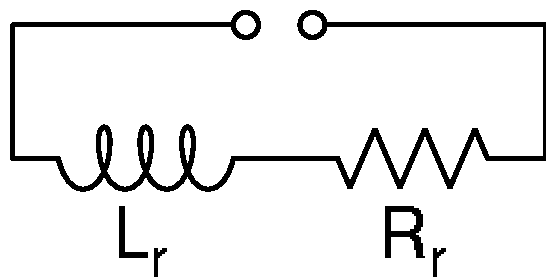
\includegraphics[width=3cm]{bilder/ersatz}}
\captionof{figure}{Ersatzschaltbild Serienschaltung}
\end{minipage}
\end{center}
\begin{align}
Z&= R+wL_r\\
|Z|&=\sqrt{R_{r}^2+(\omega L_{r})^2}\\
tan \varphi &=-\frac{\omega L_{r}}{R_{r}}
\end{align}
Analog verwendet man bei einer Parallelschaltung \((R_{p}\ und\ L_{p}) \):
\begin{center}
\begin{minipage}{\linewidth}
\centering
\makebox[0cm]{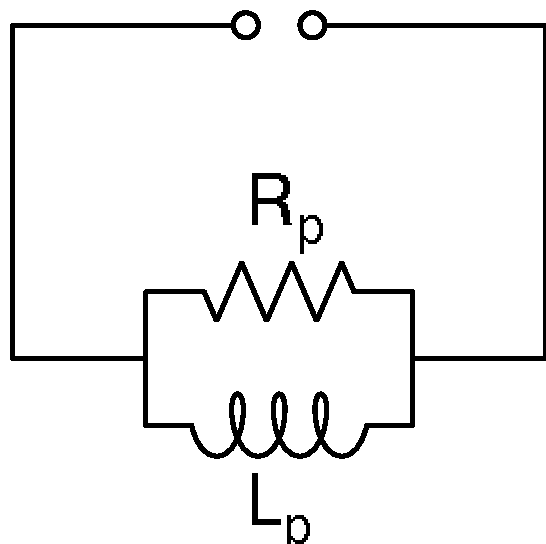
\includegraphics[width=3cm]{bilder/ersatz2}}
\captionof{figure}{Ersatzschaltbild Parallelschaltung}
\end{minipage}
\end{center}
\begin{equation}
\frac{1}{Z}=\sqrt{\frac{1}{R_{p}^2}+\frac{1}{(\omega L_{p})^2}}
\end{equation}
\begin{equation}
tan\varphi =-\frac{R_{p}}{\omega L_{p}}
\end{equation}
\subsection{Filter (Hoch-, Band-, Tiefpass)}
Die Kombinationen von R-C-L-Gliedern stellen Spannungsteiler dar.
Ein R-C-L-Bandpass ist ein schwingungsfähiges System, welches ein Impedanzminimum bei Resonanz eines Siebkreises, bzw. ein Maximum bei einem Sperrkreis aufweist.

\subsection{Wechselstrombrücke}
Eine Wechselstrombrücke (Wheatstonesche Brücke) ermöglicht die Messung von Induktivität und Kapazität, wenn die Impedanz übereinstimmt.\\
Es gilt:
\begin{equation}
\frac{L_{x}}{L_{0}}=\frac{R_{a}}{R_{b}}
\end{equation}
\begin{equation}
\frac{R_{x}+R'}{R}=\frac{R_{a}}{R_{b}}
\end{equation}
Mit dem Phasenabgleichswiderstand \(R'\) wird bei dem Bauteil die Phase verschoben.

\newpage